% Define document class
\documentclass[twocolumn]{aastex631}
\DeclareRobustCommand{\Eqref}[1]{Eq.~\ref{#1}}
\DeclareRobustCommand{\Figref}[1]{Fig.~\ref{#1}}
\DeclareRobustCommand{\Tabref}[1]{Tab.~\ref{#1}}
\DeclareRobustCommand{\Secref}[1]{Sec.~\ref{#1}}
% \usepackage{cuted}
% \usepackage{flushend}
\usepackage{amsmath}
% \graphicspath{{./figures/}}

\begin{document}

% Title
\title{Simulated Velocity Dispersion of Bar Stars in the Milky Way–M31 Merger}

\author[0009-0008-2061-4946]{C.~A.~Burt}
\affiliation{University of Arizona, Department of Astronomy \& Steward Observatory, 933 N.~Cherry Ave., Tucson, AZ 85721, USA}

\correspondingauthor{C.~A.~Burt}
\email{caburt@arizona.edu}


% \begin{abstract}
% \end{abstract}

\section{Introduction}

Galactic evolution is one of the most dynamic fields in cosmology. My
proposed topic focuses on the influence of major galactic mergers on
the bar structures in spiral galaxies. This subject encapsulates a
broader area of galaxy structure and dynamics, as it examines how the
galactic bar structure responds to dramatic changes induced by
mergers. By analyzing the evolution of these bars, we gain insight
into the mechanisms that drive the overall transformation of galaxies
\citep[e.g.,][]{vandermarel:01}.

This topic is central to our understanding of galaxy evolution because
the disruption or alteration of the bar structure plays a critical
role in the transformation of galactic geometry \citep{wu:18}. The presence
and nature of bars significantly affects star formation and the
secular evolution of galaxies \citep{schoenrich:17}. Understanding how mergers affect
these structures helps elucidate the processes that cause barred spiral
galaxies to transition into elliptical galaxies, ultimately shaping the
observable characteristics of galaxies in the universe.

Current research indicates that major galactic mergers prompt
significant changes in spiral galaxies, frequently leading to an
evolution towards an elliptical shape
\citep[e.g.,][]{mutch:11}. Although simulations have successfully
replicated some aspects of this transformation, the details of the
intermediate stages remain poorly understood \citep{berentzen:03}. The
prevailing view is that the bar structure, characteristic of many
spiral galaxies, is significantly disrupted during mergers
\citep[e.g.,][]{mutch:11}. The dynamics of stars within the bar are
disturbed, leading to a chaotic dispersal throughout the merged
galaxy. Despite a qualitative understanding of the overall process,
there exists gaps in our knowledge of the precise mechanisms at work.

Despite progress in simulating and observing galactic mergers, several
open questions persist. The exact physical measurements and
propoerties of bar structures in spiral galaxies are the subject of an
ongoing debate, which greatly influences the evolution of galactic
centers during a merger \citep{rathore:25}. Furthermore, It is partially unclear
how individual perturbations during a merger contribute to the overall
disruption of the bar, and how we can predict the detailed dynamics of
these events \citep{berentzen:03}. Addressing these uncertainties is vital for
developing a more comprehensive model of galaxy evolution post-merger,
ultimately enhancing our understanding of the lifecycle of galaxies.

\begin{figure*}[htbp]
  %\centering
  \includegraphics[width=1.0\textwidth]{dehnen23.jpeg}
  \caption{Figure 7 from \citet{dehnen:23}. The visual demonstrates
    one method used to determine the bar size and shape. This figure
    is generated from simulation snapshots, which mirrors the method I
    discuss later in the proposal.}
  \label{fig:dehnen}
\end{figure*}

\section{Proposal}

\subsection{This Proposal}
For stars ejected from the bars of the Milky Way and Andromeda (M31)
galaxies during their merger as simulated in \citet{vandermarel:12},
how does a star's initial distance from the galactic center influence
its post-merger velocity?

\subsection{Methods}
Considering sing the high-resolution simulation data from \citet{vandermarel:12},
I will write a python script that identifies the bar of the Milky Way
and M31 and tracks these stars through carefully selected snapshots
that highlight close encounters between the galaxies. This data will
then be summarized and analyzed as position-velocity phase plots and
contour maps.

To perform any analysis on the barred region of a spiral galaxy, one
must first define the bar. As previously discussed, this remains an
active area of research \citep{berentzen:03}. For this project, I
employ the method depicted in \Figref{fig:dehnen} from
\citet{dehnen:23} due to our analogous methodologies. This approach
requires an input parameter $\theta$ that I obtain from the location
of high-density regions in \Figref{fig:spiral}.

After identifying the stars located in their host galaxy's bar, I
write a function that identifies close encounters between the Milky
Way and M33 and generates a list of snapshots with an interval of 16
at ``quiet'' intervals, an interval of 1 surrounding close encounters
and interval sizes of 2, 4, and 8 to provide smooth transitions.

At each screenshot for each star located in a bar, I will generate a
scatter plot comparing the distance to the galactic center on the
x-axis to rotational velocity on the y-axis. At special snapshots
depicting the initial state, final state, and states halfway between
close encounters, I generate density contour plots from a face-down
and cylindrical perspective that portray the bar structure of the
Milky Way and M31 as well as their merger product. These plots show
allow me to address my proposal.

\begin{figure*}[htbp]
  %\centering
  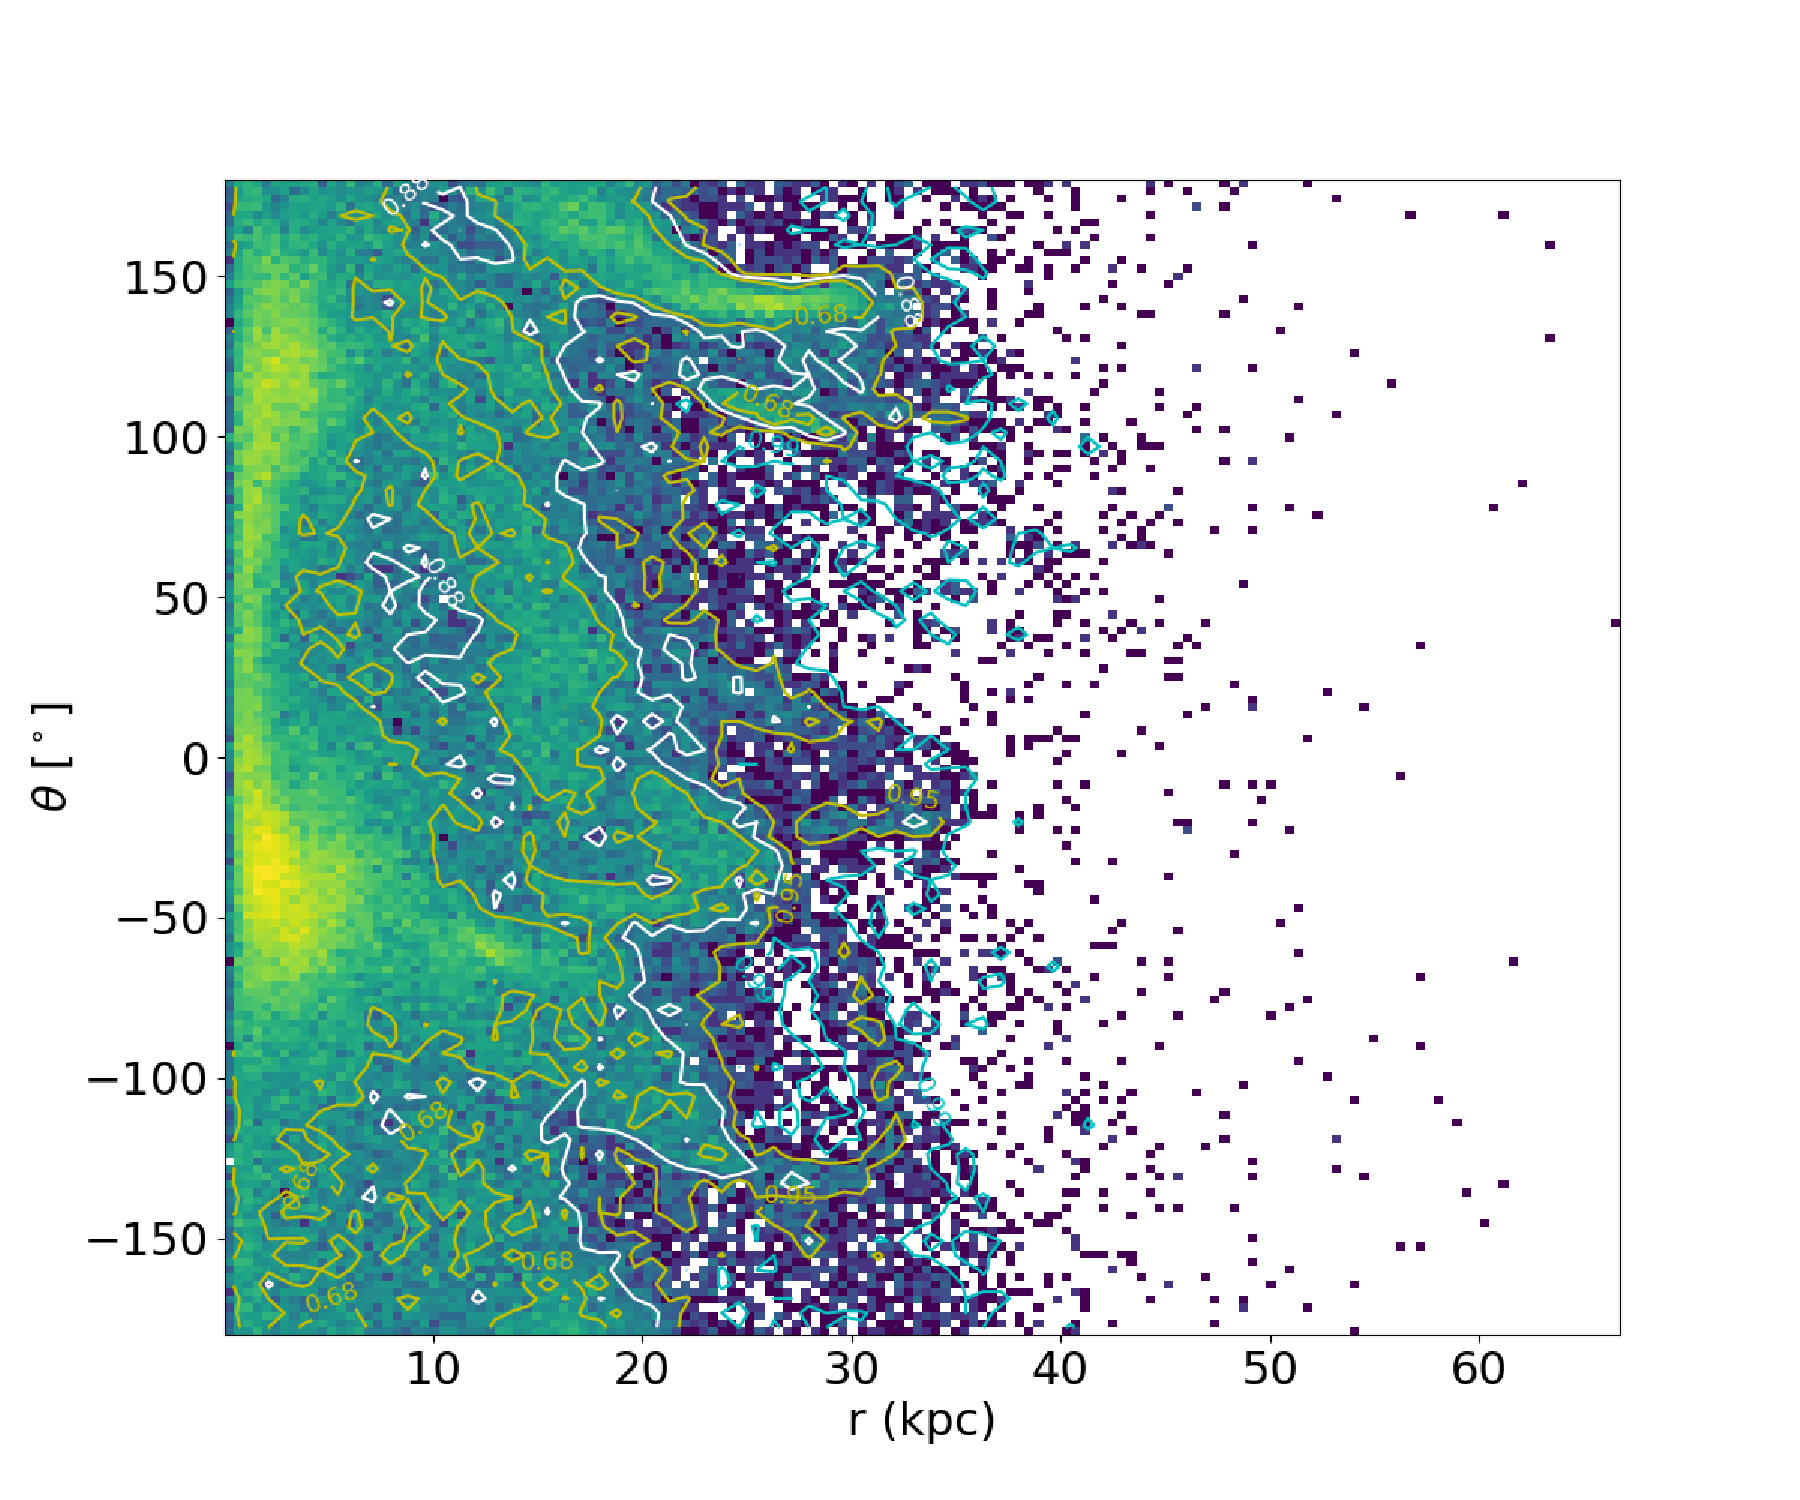
\includegraphics[width=1.0\textwidth]{Lab7_SpiralPhase}
  \caption{A histogram of M31 in polar coordinates $(r,\theta)$ onto
    $\mathbb{R}^2$ from Lab 7 from ASTR 400B Spring 2025 taught by
    Dr. G. Besla. This graph discretizes the stellar distribution,
    enabling us to identify the radius and principal angle of the
    bar. This analysis is used to determine the bar geometry for this
    project. By examining the density of the histogram, one can see
    that the bar appears most prominently at
    $\theta \approx -45^\circ$ and $\theta \approx 135^\circ$ Credit
    to G. Besla, R. Hoffman, R. Li, E. Patel, and myself for
    developing the code used to generate this figure.}
  \label{fig:spiral}
\end{figure*}

\subsection{Hypothesis}
I expect that stars initially located further from the galactic center
will exhibit higher velocities after dispersion.

\software{This work made use of the following software packages:
  \texttt{matplotlib} \citep{Hunter:2007} and \texttt{python}
  \citep{python}. Software citation information aggregated using
  \texttt{\href{https://www.tomwagg.com/software-citation-station/}{The
      Software Citation Station}}
  \citep{software-citation-station-paper,
    software-citation-station-zenodo}.}

\bibliography{./research.bib}
\end{document}

%%% Local Variables:
%%% mode: LaTeX
%%% TeX-master: t
%%% End:
